\section{Python Visualization}
\subsection{Python IQ Data Visualization}

    In this experiment, We used Python 'matplotlib.pyplot.specgram' fucntion for IQ data visualization. \\
    
    \vspace{-4mm}  
    \begin{figure}[!h]\raggedleft
    \hspace{15mm}
		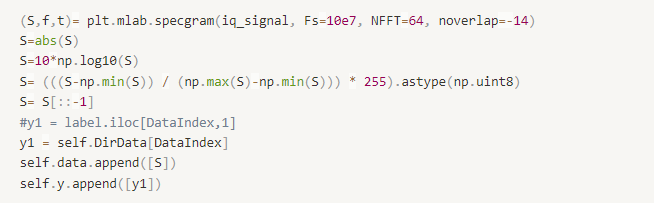
\includegraphics[width=.95\textwidth]{image/week03/1-1-1.png}
		\caption{\footnotesize Pyhton spectrogram function}
		\vspace{-10pt}
    \end{figure}
    
    The paramenters used in this function are \\
    Fs : The sampling freqeuncy used to calculate the Fourier frequencies. \\
    NFFT : The number of data points used in each block for the FFT.\\
    noverlap : The number of points of overlap between blocks.\\
    
    %%%%%%%%%%%%%%%%%%%%%%%%%%%%%%%%%%%%%%%%%%%%%%%%%
    
\subsection{IQ Data Visualization Results}

    \vspace{-4mm}  
    \begin{figure}[!h]\raggedleft
    \hspace{15mm}
		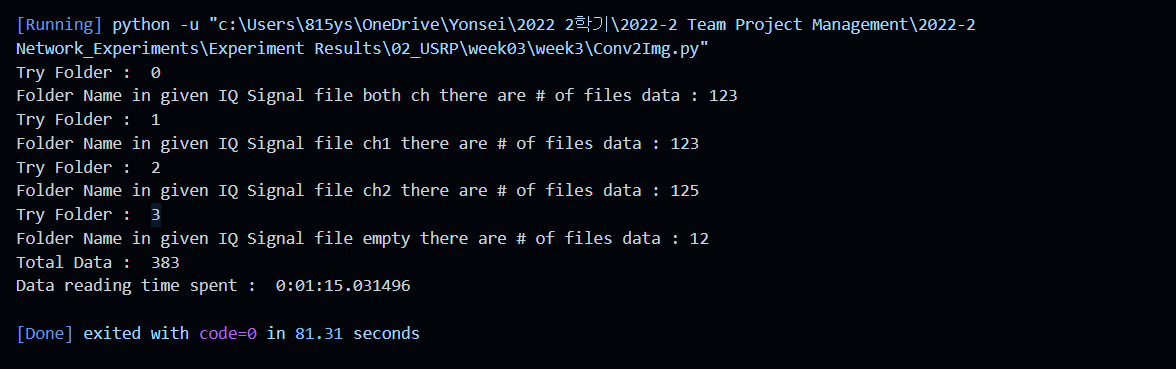
\includegraphics[width=.95\textwidth]{image/week03/1-2-1.png}
		\caption{\footnotesize IQ data visualization result}
		\vspace{-10pt}
    \end{figure}
    Using given IQ signal data, we could get 383 spectrogram images. \\
    
\clearpage